\documentclass[xcolor=dvipsnames, 9pt]{beamer}

\newenvironment{code}{\begin{semiverbatim} \begin{footnotesize}}
{\end{footnotesize}\end{semiverbatim}}

\usepackage{graphicx}
\usepackage{amssymb}
\usepackage{amsfonts}
\usepackage{amsmath}
\usepackage{hyperref}
\usepackage{natbib}
\usepackage{color}
\usepackage{pdfsync}
\usepackage{chancery}
\usepackage{movie15}
\usepackage{pgfpages}
\usepackage{fancyvrb}
\usepackage{colortbl}
\usepackage{multirow}

% \definecolor{white}{rgb}{255,255,255}
% \definecolor{darkred}{rgb}{0.5,0,0}
% \definecolor{darkgreen}{rgb}{0,0.5,0}
% \definecolor{lightblue}{rgb}{0,0,0.7}

% \hypersetup{colorlinks,
%   linkcolor=white,
%   filecolor=darkred,
%   urlcolor=lightblue,
%   citecolor=darkblue}

\usepackage{beamerthemesplit}
\usetheme{Copenhagen}
\usecolortheme[named=Violet]{structure} 
\setbeamertemplate{navigation symbols}{}
\setbeamertemplate{itemize items}[triangle]
\setbeamertemplate{enumerate items}[default]
%\setbeameroption{show notes on second screen}
% \logo{
\includegraphics[width = 2cm]{../images/logos/500px-NYU_logo.png}}

\newcommand{\R}{\mathbb{R}}
\renewcommand{\d}{\mathsf{d}}
\newcommand{\dd}{\partial}
\newcommand{\E}{\mathsf{E}}
\newcommand{\bb}{\mathbf}

\graphicspath{{../images/figures/}{../images/logos/}{../images/graphs}/}

\title{5 - Developing Algorithms}
\author{Drew Conway and Aric Hagberg}
%\institute{
\includegraphics[width = 4cm]{500px-NYU_logo.png}}
\date{June 29, 2010}

\begin{document}
\begin{frame}[plain]
\titlepage
\end{frame}

\begin{frame}
\frametitle{Outline}
\begin{itemize}
\item What is an algorithm
\item Examples of some simple algorithms
\item Writing a new algorithm
\end{itemize}
\end{frame}




\begin{frame}[fragile]
\frametitle{Feature: Compact code - building new generators}
\centerline{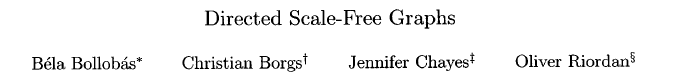
\includegraphics[width=0.7\columnwidth]{model_title}}
\centerline{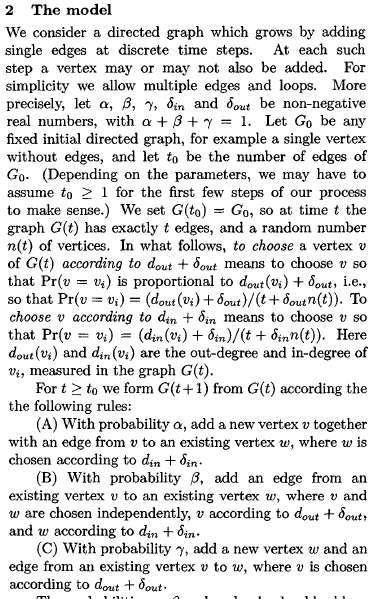
\includegraphics[width=0.4\columnwidth]{model}}
\end{frame}

\begin{frame}[fragile]
\frametitle{Feature: Compact code - building new generators}
\begin{block}{}
\tiny
\begin{verbatim}
import bisect
import random
from networkx import MultiDiGraph

def scale_free_graph(n, alpha=0.41,beta=0.54,delta_in=0.2,delta_out=0):
    def _choose_node(G,distribution,delta):
        cumsum=0.0
        psum=float(sum(distribution.values()))+float(delta)*len(distribution)
        r=random.random()
        for i in range(0,len(distribution)):
            cumsum+=(distribution[i]+delta)/psum
            if r < cumsum:  
                break
        return i

    G=MultiDiGraph()
    G.add_edges_from([(0,1),(1,2),(2,0)])
    gamma=1-alpha-beta

    while len(G)<n:
        r = random.random()
        if r < alpha:
            v = len(G) 
            w = _choose_node(G, G.in_degree(with_labels=True),delta_in)
        elif r < alpha+beta:
            v = _choose_node(G, G.out_degree(with_labels=True),delta_out)
            w = _choose_node(G, G.in_degree(with_labels=True),delta_in)
        else:
            v = _choose_node(G, G.out_degree(with_labels=True),delta_out)
            w = len(G) 
        G.add_edge(v,w)
    return G

\end{verbatim}
\end{block}
\end{frame}


% FIXME ``Expressing yourself with NetworkX''


\begin{frame}[fragile]
\frametitle{Feature: Python expressivity - a simple algorithm}
Python is easy to write and read
\begin{block}{Breadth First Search}
\begin{verbatim}
from collections import deque

def breadth_first_search(g, source):
    queue = deque([(None, source)])
    enqueued =  set([source])
    while queue:
        parent, n = queue.popleft()
        yield parent, n
        new = set(g[n]) - enqueued
        enqueued |= new
        queue.extend([(n, child) for child in new])
\end{verbatim}
\end{block}
Credit: Matteo Dell'Amico
\end{frame}



\end{document}
